\documentclass{article}

\usepackage[margin=1.5cm, includefoot, footskip=30pt]{geometry}

\usepackage[T1]{fontenc}
\usepackage{amsmath}
\usepackage{longtable,booktabs}
\usepackage{graphicx}
\usepackage{hyperref}
\usepackage{listings}
\usepackage{lmodern}
\usepackage{multicol}
\usepackage{standalone}
\usepackage{xcolor}
\usepackage{subcaption}
\usepackage{makecell}
\usepackage{authblk}
\usepackage[symbol]{footmisc}
\usepackage[sort&compress,comma,numbers]{natbib}

\usepackage{tikz}
\usetikzlibrary{calc, shapes, patterns}

\usepackage{setspace}
\renewcommand{\baselinestretch}{1.3}

\renewcommand\thesection{S\arabic{section}}

\renewcommand{\figurename}{Supplementary Figure}
\renewcommand{\tablename}{Supplementary Table}


\newcommand{\TFT}{\emph{TFT}}
\newcommand{\IPD}{\emph{IPD}}
\newcommand{\AXL}{\texttt{Axelrod-Python}}
\newcommand{\AXLFortran}{\texttt{Axelrod\_fortran}}
\newcommand{\SI}{\textbf{Supplementary Information}}

\title{Supplementary Information: Reviving, reproducing, and revisiting Axelrod's second tournament}
\author[1, $*$]{Vincent Knight}
\author[2]{Owen Campbell}
\author[3]{Marc Harper}
\author[4]{T. J. Gaffney}
\author[5, 6]{Nikoleta E. Glynatsi}

\affil[1]{School of Mathematics, Cardiff University, Cardiff, United Kingdom}
\affil[2]{Independent Researcher, Cardiff, United Kingdom}
\affil[3]{Google Inc., Mountain View, California, USA}
\affil[4]{Independent Researcher, Nevada, USA}
\affil[5]{Discrete Event Simulations Teams, RIKEN Center for Computational Science, Kobe, Japan}
\affil[6]{Mathematical Social Science Team, RIKEN Center for Interdisciplinary Theoretical and Mathematical Sciences, Wako, Japan}
\affil[$*$]{Corresponding author: KnightVA@cardiff.ac.uk.}
\date{}

\begin{document}

\maketitle

\noindent\textbf{Overview.} In this paper, we focus on reproducing Axelrod's second
tournament~\cite{Axelrod1980b}. The \SI{} provides additional
information and results that complement the main text. Namely,
it is organized as follows.

\begin{itemize}
    \item \textbf{Section~\ref{app:list_of_original_players}} lists all 63 original
    submissions, including each strategy's author and the name of its Fortran
    function in the \AXLFortran{} library.

    \item \textbf{Section~\ref{app:tournament_rankings}} reports how the original
    strategies rank across multiple tournaments considered in the paper,
    including our faithful reproduction, noisy variants, the Stewart and Plotkin
    tournament, and \AXL{} tournaments.

    \item \textbf{Section~\ref{app:reproduction_details}} provides additional
    detail on the reproduction, including the corrected Fortran source code of
    \emph{Champion} (\texttt{k61r}) and a reproduction of Axelrod's linear model.

    \item \textbf{Section~\ref{app:stewart_and_plotkin}} provides the complete
    roster and ranks for the Stewart and Plotkin tournament~\cite{Stewart2012},
    which now includes all original strategies.

    \item \textbf{Section~\ref{app:axl}} points to the full list of strategies and
    ranks for the comprehensive \AXL{} tournament (including the original
    submissions), available online.

    \item \textbf{Section~\ref{app:axl_noise}} presents the expanded \AXL{}
    tournament under 1\% and 5\% noise.

    \item \textbf{Section~\ref{app:k42r_fortran}} shows the original Fortran
    source code of \texttt{k42r} and summarizes its behavior.

    \item \textbf{Section~\ref{app:list_of_all_players}} lists all 270 original
        submissions and \AXL{} library strategies, including their rank in each
        of the new tournaments.
    \item \textbf{Section~\ref{app:opponents_distributions}} includes plots of the
    interaction distributions, in terms of cooperation rates and payoffs, for both
    the original tournament and the expanded \AXL{} tournament.
    \item \textbf{Section~\ref{app:probiblitist_distributions}} presents the
        results of the tournament under probabilistic match endings, which more
        closely reflect the intended stopping rule of Axelrod's second
        tournament.
\end{itemize}

\section{List of strategies from Axelrod's second tournament}\label{app:list_of_original_players}

Here we provide a complete list of the 63 strategies that participated in
Axelrod's second tournament. The list includes the originally reported rank of each strategy, its
author, and the name of its Fortran function implementation in the
\AXLFortran{} library.

\begin{multicols}{2}
    \begin{enumerate}
        \input{../paper/assets/list_of_original_tournament_players.tex}
    \end{enumerate}
\end{multicols}

\section{Original submissions and their tournament rankings}\label{app:tournament_rankings}

Supplementary Table~\ref{tbl:original_tournament_top_fifteen} lists the top 15
strategies from Axelrod's original tournament along with their rankings in our
reproduced tournament.

\begin{table}[!hbtp]
  \centering
  \resizebox{.9\textwidth}{!}{
    \begin{tabular}{llccccr}
\toprule
 & \makecell[c]{Author} & \makecell[c]{Average Score} & \makecell[c]{Reproduced Rank} & \makecell[c]{Original Rank} & \makecell[c]{Average\\Cooperation Rate} & \makecell[c]{Win\\proportion} \\
\midrule
k92r & Anatol Rapoport & 2.8785 & 1 & 1 & 0.9218 & 0.6306 \\
k61r & Danny C Champion & 2.7907 & 12 & 2 & 0.9542 & 0.0000 \\
k42r & Otto Borufsen & 2.8607 & 2 & 3 & 0.9161 & 0.3149 \\
k49r & Rob Cave & 2.8260 & 4 & 4 & 0.8922 & 0.0000 \\
k44r & William Adams & 2.8260 & 3 & 5 & 0.8819 & 0.0038 \\
k60r & Jim Graaskamp and Ken Katzen & 2.8102 & 9 & 6 & 0.8440 & 0.0102 \\
k41r & Herb Weiner & 2.8107 & 8 & 7 & 0.8650 & 0.0000 \\
k75r & Paul D Harrington & 2.8258 & 5 & 8 & 0.8019 & 0.0224 \\
k84r & T Nicolaus Tideman and Paula Chieruzz & 2.8124 & 7 & 9 & 0.8818 & 0.0000 \\
k32r & Charles Kluepfel & 2.8170 & 6 & 10 & 0.8726 & 0.0080 \\
k35r & Abraham Getzler & 2.8010 & 11 & 11 & 0.8878 & 0.0002 \\
k68r & Fransois Leyvraz & 2.8085 & 10 & 12 & 0.9169 & 0.0000 \\
k72r & Edward C White Jr & 2.7762 & 13 & 13 & 0.9242 & 0.0000 \\
k46r & Graham J Eatherley & 2.7722 & 14 & 14 & 0.9483 & 0.0000 \\
k83r & Paul E Black & 2.7425 & 15 & 15 & 0.9347 & 0.0000 \\
\bottomrule
\end{tabular}
}
  \caption{\textbf{Top 15 strategies in the reproduced tournament.}
  The table lists the top 15 strategies from Axelrod's original tournament
  along with their rankings in our reproduced tournament. For each strategy, we
  report the average score and the average cooperation rate in the reproduced
  tournament, as well as the proportion of wins across our repetitions of the
  original tournament. \TFT{} wins 63.3\% of these repetitions, indicating that
  in 36.7\% of runs a different winner emerges.}
  \label{tbl:original_tournament_top_fifteen}
\end{table}

For the original strategies, we evaluate performance in the following
tournaments:
\begin{itemize}
    \item \textbf{Reproduced tournament:} A faithful reproduction of Axelrod's second tournament.
    \item \textbf{Noisy tournament:} The original tournament with a noise (error) probability of 0.01.
    \item \textbf{Stewart and Plotkin tournament~\cite{Stewart2012}:} A tournament with the original submission and the submissions used by Stewart \& Plotkin.
    \item \textbf{\AXL{} tournament:} A tournament including all strategies from the \AXL{} library and the original submissions.
    \item \textbf{\AXL{} tournament with 1\% noise:} As above, with 1\% noise.
    \item \textbf{\AXL{} tournament with 5\% noise:} As above, with 5\% noise.
\end{itemize}

Supplementary Table~\ref{tbl:original_tournament_rankings_all_tournaments} shows
the strategies and their ranks across these tournaments.

\begin{table}[!hbtp]
    \resizebox{\textwidth}{!}{
    \centering
    \begin{tabular}{lccccccc}
\toprule
 & \makecell[c]{Original\\Rank} & \makecell[c]{Reproduced\\Rank} & \makecell[c]{Reproduced Rank\\(Noise 1\%)} & \makecell[c]{S \& P\\tournament Rank} & \makecell[c]{AXL\\tournament Rank} & \makecell[c]{AXL (Noise 1\%)\\tournament Rank} & \makecell[c]{AXL (Noise 5\%)\\tournament Rank} \\
\midrule
k92r & 1 & 1 & 28 & 4 & 57 & 70 & 69 \\
k61r & 2 & 12 & 44 & 8 & 85 & 126 & 156 \\
k42r & 3 & 2 & 8 & 2 & 16 & 25 & 21 \\
k49r & 4 & 4 & 12 & 5 & 30 & 32 & 23 \\
k44r & 5 & 3 & 16 & 7 & 46 & 37 & 26 \\
k60r & 6 & 9 & 11 & 16 & 19 & 31 & 25 \\
k41r & 7 & 8 & 13 & 10 & 35 & 33 & 40 \\
k75r & 8 & 5 & 20 & 6 & 110 & 42 & 31 \\
k84r & 9 & 7 & 21 & 15 & 47 & 43 & 76 \\
k32r & 10 & 6 & 18 & 12 & 23 & 40 & 34 \\
k35r & 11 & 11 & 36 & 14 & 87 & 95 & 89 \\
k68r & 12 & 10 & 41 & 9 & 66 & 117 & 139 \\
k72r & 13 & 13 & 32 & 13 & 78 & 77 & 38 \\
k46r & 14 & 14 & 26 & 11 & 74 & 63 & 77 \\
k83r & 15 & 15 & 35 & 17 & 106 & 92 & 83 \\
k47r & 16 & 16 & 4 & 22 & 84 & 16 & 5 \\
k64r & 17 & 17 & 29 & 18 & 92 & 71 & 46 \\
k51r & 18 & 19 & 54 & 30 & 164 & 167 & 158 \\
k78r & 19 & 20 & 33 & 37 & 145 & 80 & 61 \\
k66r & 20 & 18 & 19 & 19 & 71 & 41 & 19 \\
k58r & 21 & 21 & 17 & 23 & 25 & 38 & 43 \\
k88r & 22 & 22 & 43 & 25 & 126 & 122 & 113 \\
k31r & 23 & 23 & 39 & 24 & 127 & 107 & 73 \\
k90r & 24 & 26 & 38 & 27 & 132 & 104 & 71 \\
k39r & 25 & 27 & 34 & 21 & 130 & 81 & 20 \\
k79r & 26 & 24 & 23 & 26 & 88 & 52 & 54 \\
k67r & 27 & 25 & 37 & 28 & 146 & 103 & 33 \\
k86r & 28 & 30 & 15 & 33 & 67 & 36 & 49 \\
k69r & 29 & 31 & 42 & 43 & 144 & 121 & 48 \\
k91r & 30 & 28 & 27 & 29 & 89 & 67 & 52 \\
k57r & 31 & 29 & 49 & 40 & 115 & 147 & 182 \\
k70r & 32 & 35 & 46 & 41 & 104 & 129 & 149 \\
k85r & 33 & 37 & 24 & 47 & 20 & 57 & 101 \\
k38r & 34 & 33 & 9 & 34 & 51 & 26 & 7 \\
k40r & 35 & 32 & 14 & 38 & 27 & 34 & 80 \\
k80r & 36 & 34 & 3 & 31 & 22 & 10 & 3 \\
k37r & 37 & 42 & 30 & 44 & 113 & 73 & 57 \\
k56r & 38 & 41 & 6 & 36 & 31 & 21 & 12 \\
k43r & 39 & 38 & 5 & 32 & 79 & 18 & 6 \\
k59r & 40 & 40 & 7 & 35 & 32 & 23 & 11 \\
k73r & 41 & 44 & 22 & 42 & 101 & 44 & 50 \\
k55r & 42 & 43 & 10 & 39 & 36 & 27 & 15 \\
k81r & 43 & 45 & 2 & 45 & 43 & 6 & 14 \\
k87r & 44 & 39 & 31 & 46 & 26 & 74 & 124 \\
k53r & 45 & 46 & 45 & 49 & 99 & 128 & 128 \\
k76r & 46 & 36 & 53 & 48 & 155 & 166 & 155 \\
k65r & 47 & 48 & 1 & 50 & 28 & 5 & 18 \\
k52r & 48 & 47 & 50 & 51 & 169 & 151 & 100 \\
k82r & 49 & 50 & 25 & 56 & 148 & 58 & 28 \\
k45r & 50 & 49 & 52 & 55 & 163 & 159 & 115 \\
k62r & 51 & 51 & 51 & 57 & 173 & 158 & 99 \\
k34r & 52 & 52 & 40 & 58 & 83 & 111 & 119 \\
k48r & 53 & 53 & 48 & 60 & 151 & 141 & 94 \\
k50r & 54 & 54 & 60 & 62 & 240 & 235 & 249 \\
k77r & 55 & 55 & 47 & 64 & 170 & 131 & 45 \\
k89r & 56 & 56 & 58 & 63 & 175 & 200 & 191 \\
k63r & 57 & 58 & 61 & 67 & 230 & 240 & 248 \\
k54r & 58 & 57 & 57 & 65 & 191 & 191 & 143 \\
k33r & 59 & 59 & 55 & 66 & 166 & 178 & 145 \\
k71r & 60 & 60 & 59 & 68 & 219 & 222 & 220 \\
k74r & 61 & 61 & 56 & 69 & 190 & 186 & 120 \\
krandomc & 62 & 62 & 63 & 71 & 260 & 252 & 255 \\
k36r & 63 & 63 & 62 & 72 & 247 & 251 & 243 \\
\bottomrule
\end{tabular}
}
    \caption{\textbf{Ranks of the original strategies across different tournaments.}}
    \label{tbl:original_tournament_rankings_all_tournaments}
\end{table}


\section{Reproducing Champion and Axelrod's linear model}\label{app:reproduction_details}

Here we provide additional detail on the reproduction of Axelrod's second
tournament. Supplementary Figure~\ref{fig:champion_fortran} shows the corrected
Fortran source code of \emph{Champion} (\texttt{k61r}), and
Supplementary Figure~\ref{fig:linear_regression} reproduces Axelrod's linear
model relating strategy features to average score.

\begin{figure}[!hbtp]
    \begin{center}
        \begin{lstlisting}[language=Fortran,
                           basicstyle=\ttfamily\scriptsize,
                           frame=single,
                           keywordstyle=\color{red}\bfseries,
                           commentstyle=\color{teal}\itshape]
      FUNCTION K61R(ISPICK,ITURN,K,L,R, JA)
C BY DANNY C. CHAMPION
C TYPED BY JM 3/27/79
      k61r=ja    ! Added 7/27/93 to report own old value
      IF (ITURN .EQ. 1) ICOOP = 0  ! Added 10/8/2017 to fix bug for multiple runs
      IF (ITURN .EQ. 1) K61R = 0
      IF (ISPICK .EQ. 0) ICOOP = ICOOP + 1
      IF (ITURN .LE. 10) RETURN
      K61R = ISPICK
      IF (ITURN .LE. 25) RETURN
      K61R = 0
      COPRAT = FLOAT(ICOOP) / FLOAT(ITURN)
      IF (ISPICK .EQ. 1 .AND. COPRAT .LT. .6 .AND. R .GT. COPRAT)
     +K61R = 1
      RETURN
      END
        \end{lstlisting}
    \caption{\textbf{Fortran source code for \texttt{k61r} (Champion).}
    The original implementation contained a bug: the variable \texttt{ICOOP} was not
    initialized within the function. In the first match it effectively started at 0,
    but in subsequent matches it could have kept its value from the previous match or be reset to 0,
    depending on the compiler and runtime environment. Line~5 shows the fix, which
    explicitly initializes \texttt{ICOOP} at the start of each match.}
    \label{fig:champion_fortran}
    \end{center}
\end{figure}


\begin{figure}[!hbtp]
    \centering
    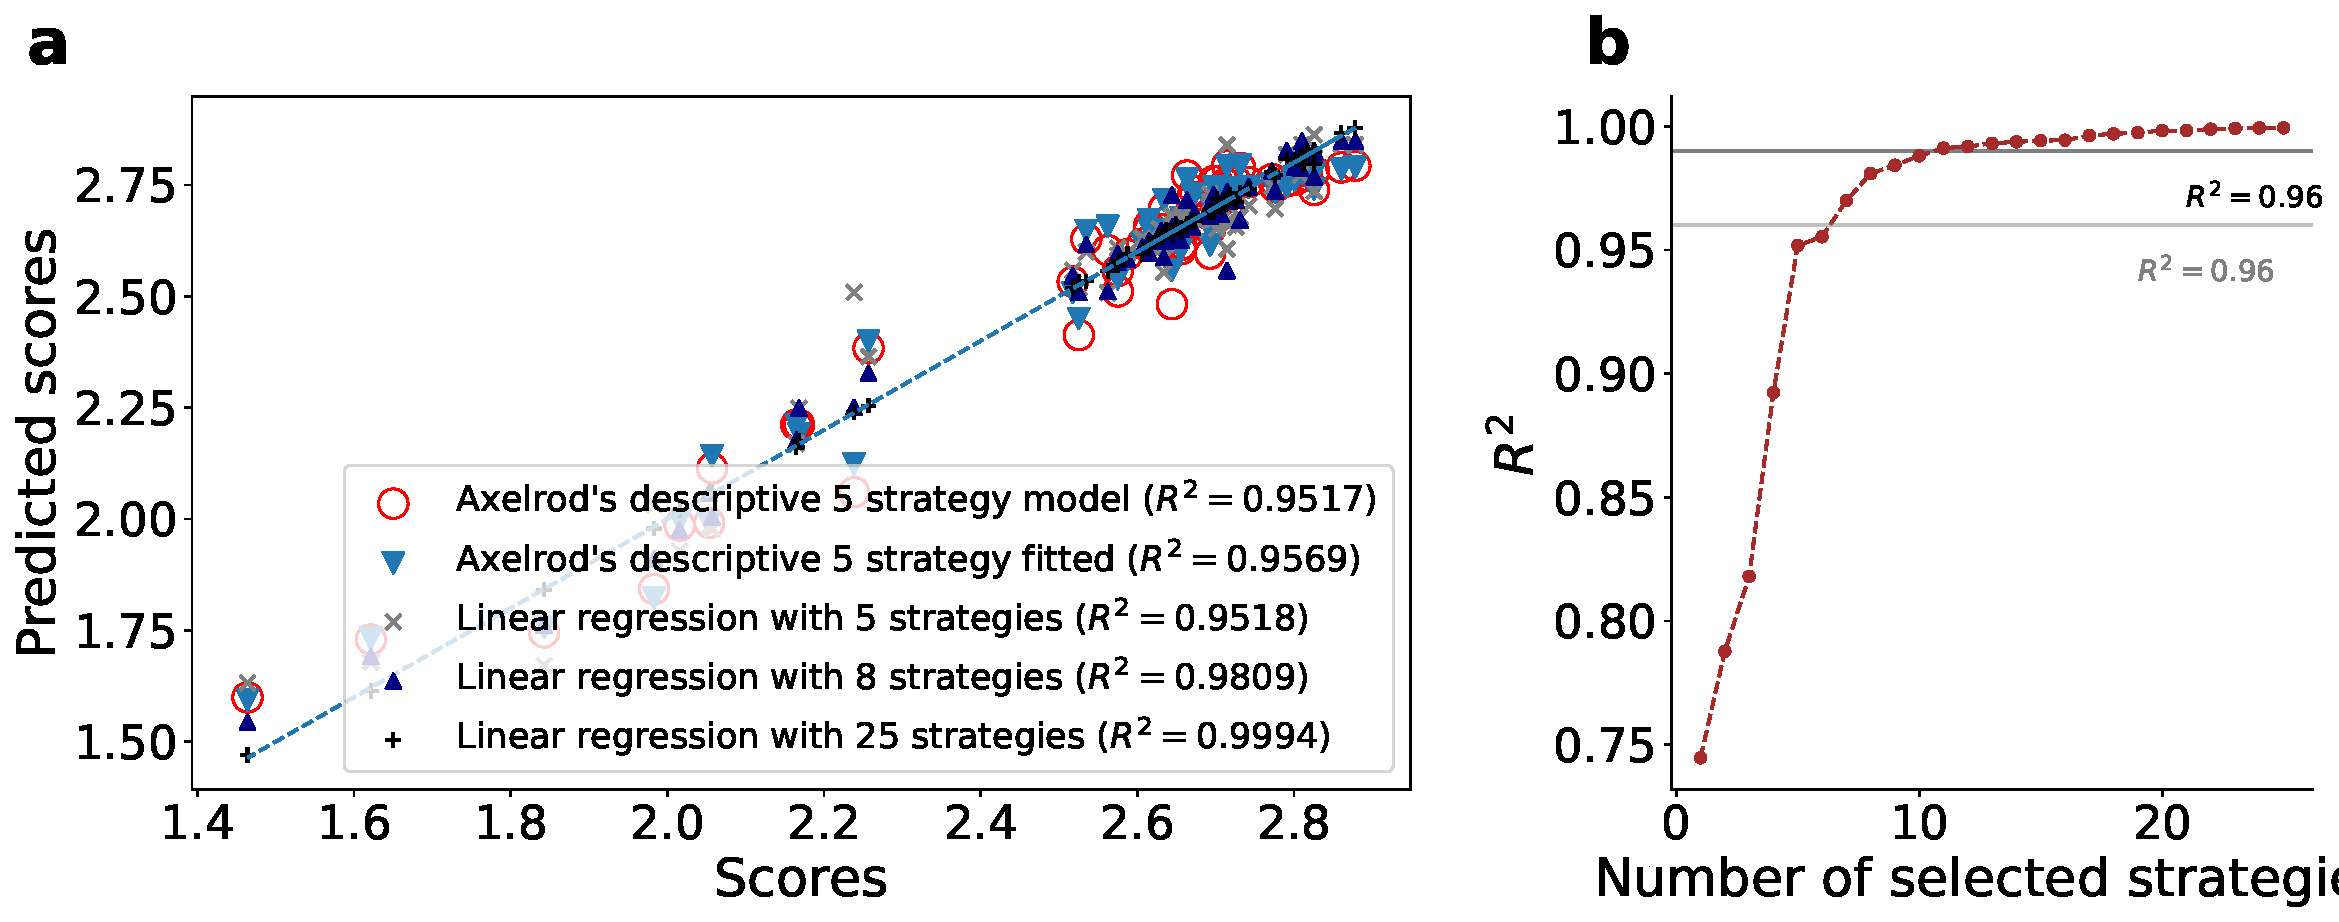
\includegraphics[width=\textwidth]{../paper/assets/Figure_linear_regression_results.pdf}
    \caption{\textbf{Reproduction of Axelrod's linear model.}
    \textbf{a,} The representative strategies and their effect on average score.
    We reproduce the linear model described in~\cite{Axelrod1980b}, which reports
    \(R^2 = 0.979\). Fitting a new model to the same five strategies yields
    \(R^2 = \protect\input{../paper/assets/original_tournament_predictive_with_axelrod_5_r_squared.tex}\).
    The fit is an ordinary least squares linear regression; the reported \(R^2\)
    values are coefficients of determination, and no significance tests or
    multiple-comparison adjustments were applied.
    \textbf{b,} \(R^2\) as a function of the number of strategies included (subset size),
    obtained using recursive feature elimination (RFE)~\cite{guyon2002gene}.
    Starting from the full set of strategies, we iteratively remove the least
    informative one, refit the model, and record the resulting \(R^2\).
    For each subset size (from 1 to 25), the subset yielding the highest \(R^2\)
    is retained. The estimated \(R^2\) rises rapidly from about 0.75 to 0.95 as
    the number of included strategies increases from 1 to 5, after which
    improvements are smaller.}
    \label{fig:linear_regression}
\end{figure}


\section{Full list of strategies and ranks of Stewart and Plotkin tournament}\label{app:stewart_and_plotkin}

Supplementary Table~\ref{tbl:sp_tournament_top_fifteen} reports the top 15
strategies in the Stewart and Plotkin tournament~\cite{Stewart2012}, and
Supplementary Table~\ref{tbl:sp_tournament_full_rankings} gives the full list of
strategies and their ranks in that tournament, which now includes the original
strategies.

\begin{table}[!hbtp]
        \centering
        \resizebox{.8\textwidth}{!}{
        \begin{tabular}{lccccc}
\toprule
 & \makecell[c]{Average\\Score} & \makecell[c]{Rank} & \makecell[c]{Average\\Cooperation Rate} & \makecell[c]{Reproduced Average\\Cooperation Rate} & \makecell[c]{S. and P. Average\\Cooperation Rate} \\
Name &  &  &  &  &  \\
\midrule
ZD-GTFT-2: 0.25, 0.5 & 2.834 & 1 & 0.926 & - & 0.855 \\
k42r & 2.825 & 2 & 0.903 & 0.916 & - \\
GTFT: 0.33 & 2.819 & 3 & 0.941 & - & 0.893 \\
k92r & 2.812 & 4 & 0.888 & 0.922 & 0.731 \\
k49r & 2.787 & 5 & 0.879 & 0.892 & - \\
k75r & 2.786 & 6 & 0.782 & 0.802 & - \\
k44r & 2.781 & 7 & 0.866 & 0.882 & - \\
k61r & 2.773 & 8 & 0.945 & 0.954 & - \\
k68r & 2.768 & 9 & 0.904 & 0.917 & - \\
k41r & 2.761 & 10 & 0.847 & 0.865 & - \\
k46r & 2.758 & 11 & 0.939 & 0.948 & - \\
k32r & 2.758 & 12 & 0.849 & 0.873 & - \\
k72r & 2.756 & 13 & 0.915 & 0.924 & - \\
k35r & 2.747 & 14 & 0.863 & 0.888 & - \\
k84r & 2.745 & 15 & 0.861 & 0.882 & - \\
\bottomrule
\end{tabular}
}
        \caption{\textbf{Top 15 strategies in the Stewart and Plotkin tournament.}
        We report the mean score, rank, and mean cooperation rate. For comparison,
        we also include the cooperation rate from our reproduced tournament,
        alongside the cooperation rates originally reported by Stewart and Plotkin.}
        \label{tbl:sp_tournament_top_fifteen}
\end{table}

\begin{table}[!hbtp]
        \resizebox{\textwidth}{.5\textheight}{
        \centering
        \begin{tabular}{lccccc}
\toprule
 & \makecell[c]{Mean Score} & \makecell[c]{Rank} & \makecell[c]{Mean\\Cooperation Rate} & \makecell[c]{Reproduced Mean\\Cooperation Rate} & \makecell[c]{S. and P. Mean\\Cooperation Rate} \\
\midrule
ZD-GTFT-2: 0.25, 0.5 & 2.834 & 1 & 0.926 & - & 0.855 \\
k42r & 2.825 & 2 & 0.903 & 0.916 & - \\
GTFT: 0.33 & 2.819 & 3 & 0.941 & - & 0.893 \\
k92r & 2.812 & 4 & 0.888 & 0.922 & 0.731 \\
k49r & 2.787 & 5 & 0.879 & 0.892 & - \\
k75r & 2.786 & 6 & 0.782 & 0.802 & - \\
k44r & 2.781 & 7 & 0.866 & 0.882 & - \\
k61r & 2.773 & 8 & 0.945 & 0.954 & - \\
k68r & 2.768 & 9 & 0.904 & 0.917 & - \\
k41r & 2.761 & 10 & 0.847 & 0.865 & - \\
k46r & 2.758 & 11 & 0.939 & 0.948 & - \\
k32r & 2.758 & 12 & 0.849 & 0.873 & - \\
k72r & 2.756 & 13 & 0.915 & 0.924 & - \\
k35r & 2.747 & 14 & 0.863 & 0.888 & - \\
k84r & 2.745 & 15 & 0.861 & 0.882 & - \\
k60r & 2.735 & 16 & 0.814 & 0.844 & - \\
k83r & 2.725 & 17 & 0.922 & 0.935 & - \\
k64r & 2.710 & 18 & 0.876 & 0.884 & - \\
k66r & 2.702 & 19 & 0.861 & 0.866 & - \\
Hard Tit For 2 Tats & 2.701 & 20 & 0.926 & - & 0.807 \\
k39r & 2.700 & 21 & 0.671 & 0.676 & - \\
k47r & 2.696 & 22 & 0.709 & 0.723 & - \\
k58r & 2.694 & 23 & 0.846 & 0.852 & - \\
k31r & 2.690 & 24 & 0.908 & 0.920 & - \\
k88r & 2.684 & 25 & 0.851 & 0.861 & - \\
k79r & 2.678 & 26 & 0.864 & 0.875 & - \\
k90r & 2.676 & 27 & 0.943 & 0.964 & 0.844 \\
k67r & 2.676 & 28 & 0.743 & 0.749 & - \\
k91r & 2.662 & 29 & 0.889 & 0.873 & - \\
k51r & 2.646 & 30 & 0.892 & 0.905 & - \\
k80r & 2.641 & 31 & 0.813 & 0.809 & - \\
k43r & 2.641 & 32 & 0.673 & 0.666 & - \\
k86r & 2.639 & 33 & 0.803 & 0.811 & - \\
k38r & 2.639 & 34 & 0.865 & 0.874 & - \\
k59r & 2.635 & 35 & 0.889 & 0.891 & - \\
k56r & 2.635 & 36 & 0.890 & 0.891 & - \\
k78r & 2.634 & 37 & 0.720 & 0.755 & - \\
k40r & 2.625 & 38 & 0.742 & 0.746 & - \\
k55r & 2.620 & 39 & 0.903 & 0.903 & - \\
k57r & 2.620 & 40 & 0.799 & 0.811 & - \\
k70r & 2.596 & 41 & 0.752 & 0.769 & - \\
k73r & 2.595 & 42 & 0.761 & 0.764 & - \\
k69r & 2.591 & 43 & 0.672 & 0.702 & - \\
k37r & 2.590 & 44 & 0.778 & 0.791 & - \\
k81r & 2.589 & 45 & 0.774 & 0.779 & - \\
k87r & 2.586 & 46 & 0.760 & 0.766 & - \\
k85r & 2.584 & 47 & 0.713 & 0.726 & - \\
k76r & 2.576 & 48 & 0.636 & 0.680 & - \\
k53r & 2.568 & 49 & 0.730 & 0.728 & - \\
k65r & 2.559 & 50 & 0.718 & 0.715 & - \\
k52r & 2.545 & 51 & 0.820 & 0.838 & - \\
Win-Stay Lose-Shift & 2.544 & 52 & 0.809 & - & 0.808 \\
Hard Tit For Tat & 2.539 & 53 & 0.710 & - & 0.663 \\
Cooperator & 2.522 & 54 & 1.000 & - & 1.000 \\
k45r & 2.521 & 55 & 0.726 & 0.754 & - \\
k82r & 2.491 & 56 & 0.529 & 0.544 & - \\
k62r & 2.490 & 57 & 0.732 & 0.754 & - \\
k34r & 2.478 & 58 & 0.647 & 0.652 & 0.655 \\
Hard Go By Majority & 2.375 & 59 & 0.658 & - & 0.459 \\
k48r & 2.300 & 60 & 0.504 & 0.499 & - \\
First by Joss: 0.9 & 2.280 & 61 & 0.501 & - & 0.345 \\
k50r & 2.248 & 62 & 0.929 & 0.930 & - \\
k89r & 2.212 & 63 & 0.504 & 0.498 & - \\
k77r & 2.165 & 64 & 0.327 & 0.332 & - \\
k54r & 2.118 & 65 & 0.483 & 0.467 & - \\
k33r & 2.108 & 66 & 0.424 & 0.411 & - \\
k63r & 2.096 & 67 & 0.502 & 0.502 & - \\
k71r & 2.032 & 68 & 0.166 & 0.158 & - \\
k74r & 1.881 & 69 & 0.171 & 0.174 & - \\
ZD-Extort-2: 0.1111111111111111, 0.5 & 1.838 & 70 & 0.254 & - & 0.232 \\
krandomc & 1.698 & 71 & 0.500 & 0.500 & 0.500 \\
k36r & 1.520 & 72 & 0.092 & 0.092 & - \\
Defector & 1.472 & 73 & 0.000 & - & 0.000 \\
\bottomrule
\end{tabular}
}
        \caption{Stewart and Plotkin tournament full list of rankings.}
        \label{tbl:sp_tournament_full_rankings}
\end{table}


\section{Full list of strategies and ranks for \AXL{} tournament}\label{app:axl}

The full list of strategies and their ranks in the \AXL{} tournament, which now
includes the original strategies, can be found online at
\url{https://github.com/Axelrod-Python/tournament}.
This includes tournaments with and without noise.
Supplementary Table~\ref{tbl:axl_tournament_top_sixteen} reports the top 16
strategies in this tournament.

\begin{table}[!hbtp]
    \centering
    \resizebox{.9\textwidth}{!}{
    \begin{tabular}{lccccccc}
\toprule
 & \makecell[c]{Average\\Score} & \makecell[c]{Rank} & \makecell[c]{Average\\Cooperation Rate} & \makecell[c]{Original Rank} & \makecell[c]{Reproduced Average\\Cooperation Rate} & \makecell[c]{Library Rank} & \makecell[c]{Library Average\\Cooperation Rate} \\
\midrule
EvolvedLookerUp2\_2\_2\textsuperscript{\textdagger} & 2.802 & 1 & 0.756 & - & - & 1 & 0.736 \\
Evolved HMM 5\textsuperscript{\textdagger} & 2.788 & 2 & 0.751 & - & - & 2 & 0.742 \\
Omega TFT: 3, 8 & 2.786 & 3 & 0.750 & - & - & 12 & 0.725 \\
Evolved ANN 5\textsuperscript{\textdagger} & 2.784 & 4 & 0.720 & - & - & 3 & 0.713 \\
Evolved ANN\textsuperscript{\textdagger} & 2.782 & 5 & 0.739 & - & - & 5 & 0.727 \\
Evolved FSM 16\textsuperscript{\textdagger} & 2.780 & 6 & 0.731 & - & - & 4 & 0.713 \\
Evolved FSM 16 Noise 05\textsuperscript{\textdagger} & 2.776 & 7 & 0.726 & - & - & 6 & 0.717 \\
PSO Gambler 2\_2\_2\textsuperscript{\textdagger} & 2.760 & 8 & 0.702 & - & - & 7 & 0.692 \\
Original Gradual & 2.757 & 9 & 0.808 & - & - & - & - \\
PSO Gambler 2\_2\_2 Noise 05\textsuperscript{\textdagger} & 2.756 & 10 & 0.740 & - & - & 14 & 0.723 \\
PSO Gambler Mem1\textsuperscript{\textdagger} & 2.756 & 11 & 0.734 & - & - & 9 & 0.728 \\
Evolved FSM 4\textsuperscript{\textdagger} & 2.752 & 12 & 0.793 & - & - & 10 & 0.777 \\
PSO Gambler 1\_1\_1\textsuperscript{\textdagger} & 2.752 & 13 & 0.704 & - & - & 8 & 0.702 \\
Gradual & 2.746 & 14 & 0.763 & - & - & 15 & 0.793 \\
DBS: 0.75, 3, 4, 3, 5 & 2.739 & 15 & 0.750 & - & - & 11 & 0.739 \\
k42r & 2.735 & 16 & 0.820 & 3 & 0.916 & - & - \\
\bottomrule
\end{tabular}
}
    \caption{\textbf{Top 16 strategies in the \AXL{} tournament.} This
    tournament includes all strategies from the \AXL{} library alongside the
    original Fortran strategies. In total, there are 272 strategies competing.
    Strategies denoted by $^\dagger$ were not designed but, they were trained
    via reinforcement learning, as described in~\cite{Harper2017}.}
    \label{tbl:axl_tournament_top_sixteen}
\end{table}


\section{The expanded \AXL{} tournament under noise}\label{app:axl_noise}

We repeat the expanded \AXL{} tournament under noise, where with a fixed
probability each intended action is flipped. Supplementary
Figure~\ref{fig:axl_noise_1} shows the results under 1\% noise and
Supplementary Figure~\ref{fig:axl_noise_5} under 5\% noise. As expected, noise
reduces the advantage of highly cooperative strategies, but the overall
structure of the tournament is preserved.

\begin{figure}[!hbtp]
    \centering
    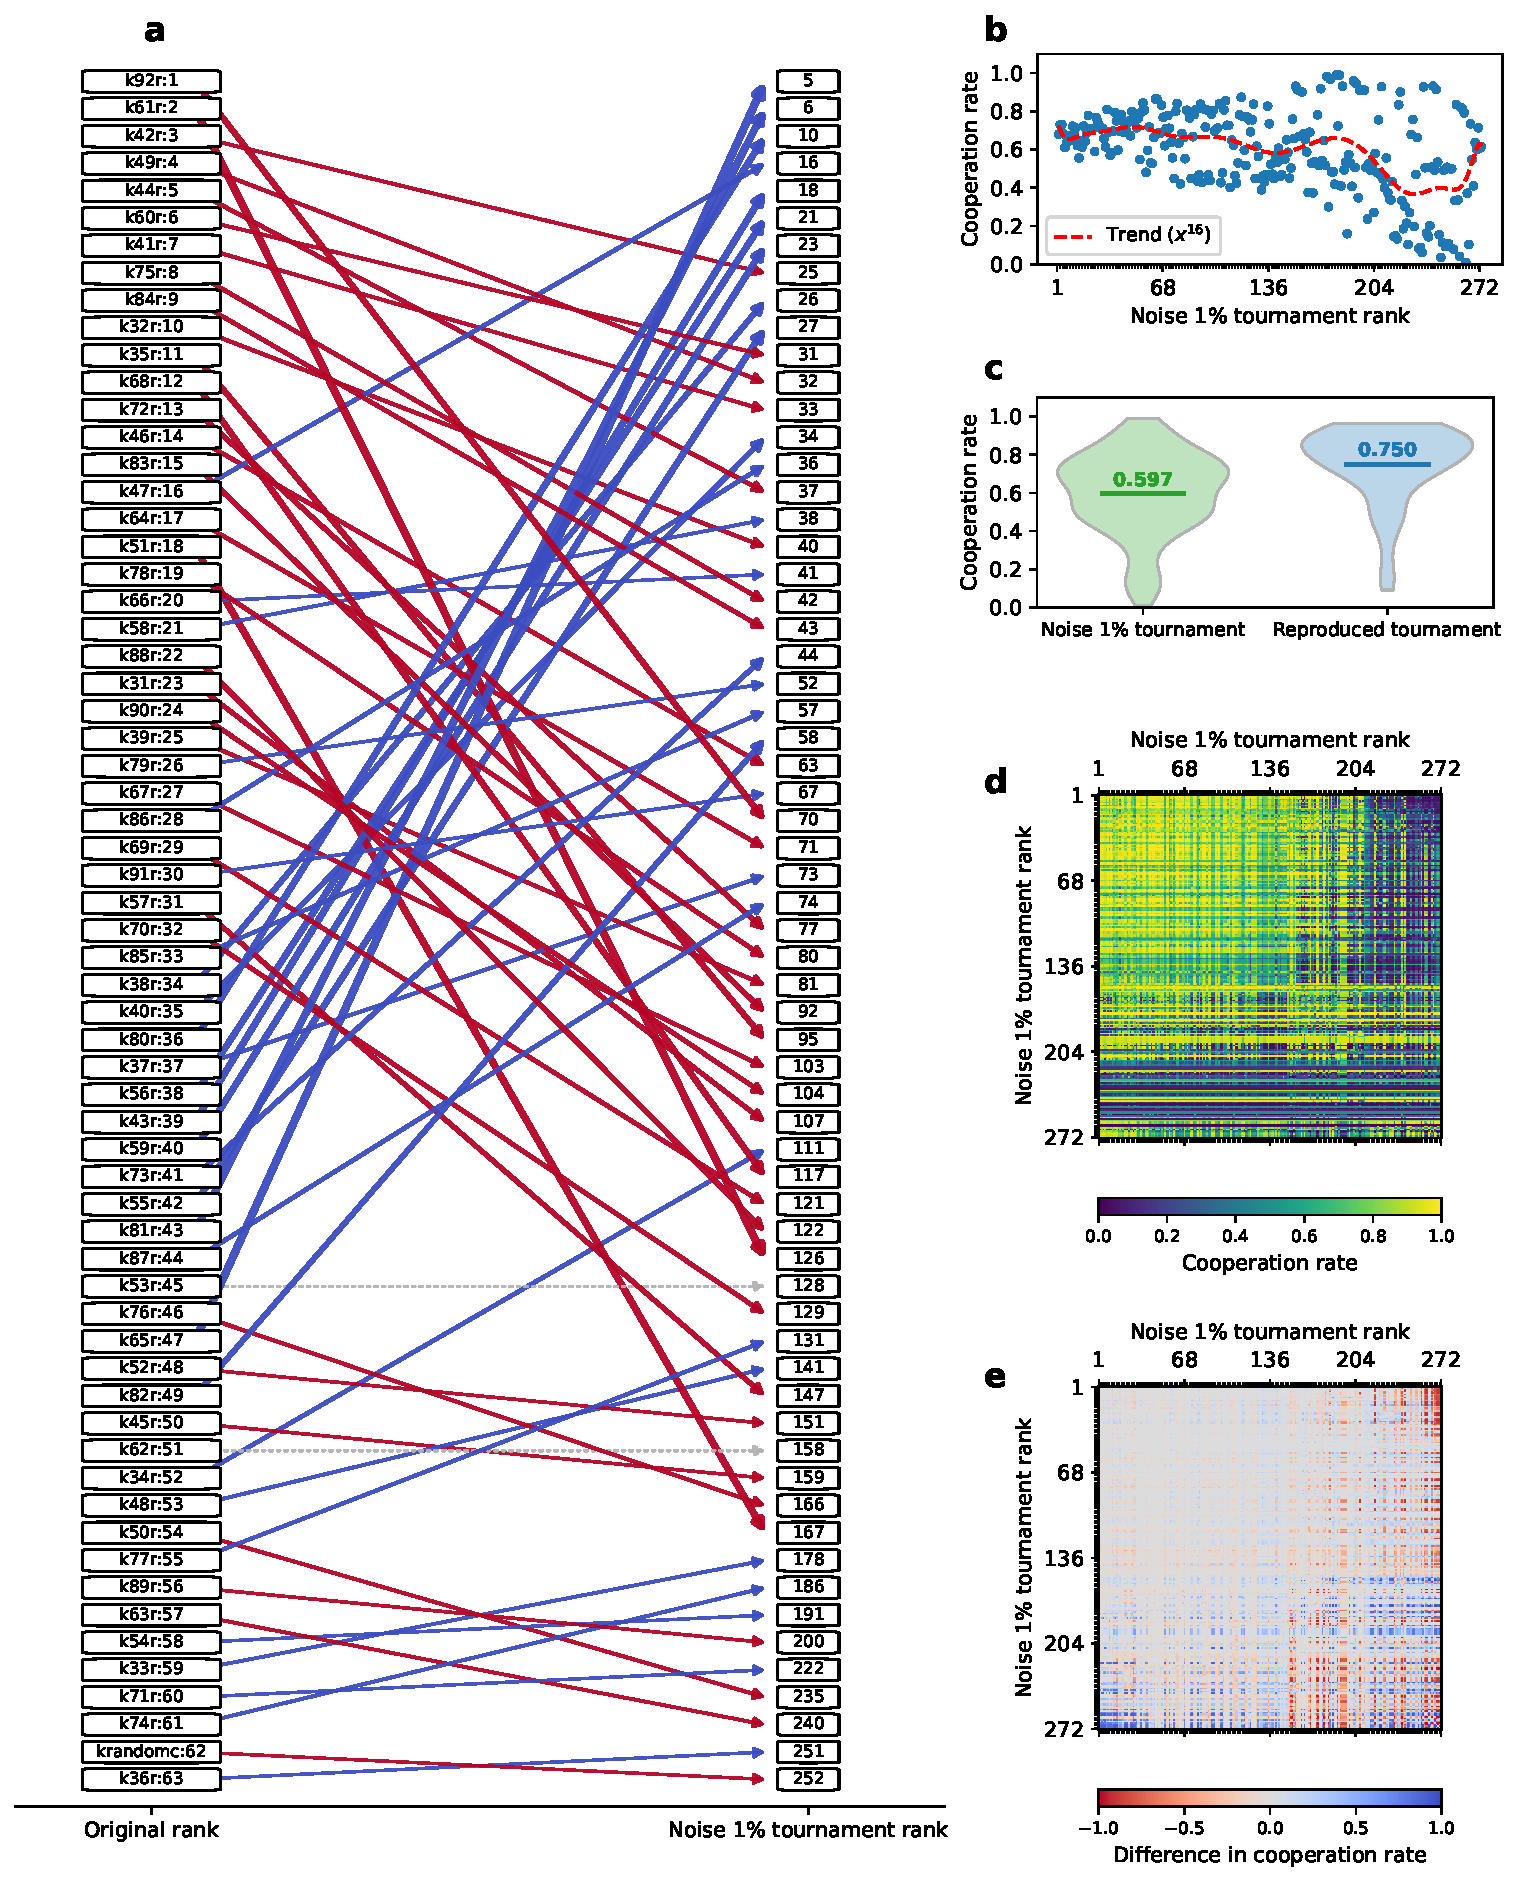
\includegraphics[width=.90\textwidth]{../paper/assets/axelrod_python_tournament_noise_1.pdf}
    \caption{\textbf{Reproduction of Axelrod's second tournament with the addition
    of the strategies from the \AXL{} library and 1\% noise.}
    \textbf{a,} Comparison of the original rankings (left column) and the rankings
    in this tournament (right column), with strategies ordered by their original
    ranks. Arrows indicate the change in rank, with widths proportional to the size
    of the change; blue arrows indicate a positive change in rank, red arrows a
    negative change, and grey arrows no change.
    \textbf{b,} Cooperation rates of strategies ordered by rank in this tournament.
    \textbf{c,} Tournament cooperation rates across all repetitions for this
    tournament (green) and the reproduced tournament without the additional
    strategies (blue); the solid line shows the average cooperation rate.
    \textbf{d,} Pairwise cooperation rates between strategies, ordered by their
    rank in this tournament.
    \textbf{e,} Differences in pairwise cooperation rates, again ordered by rank
    in this tournament.}
    \label{fig:axl_noise_1}
\end{figure}


\begin{figure}[!hbtp]
    \centering
    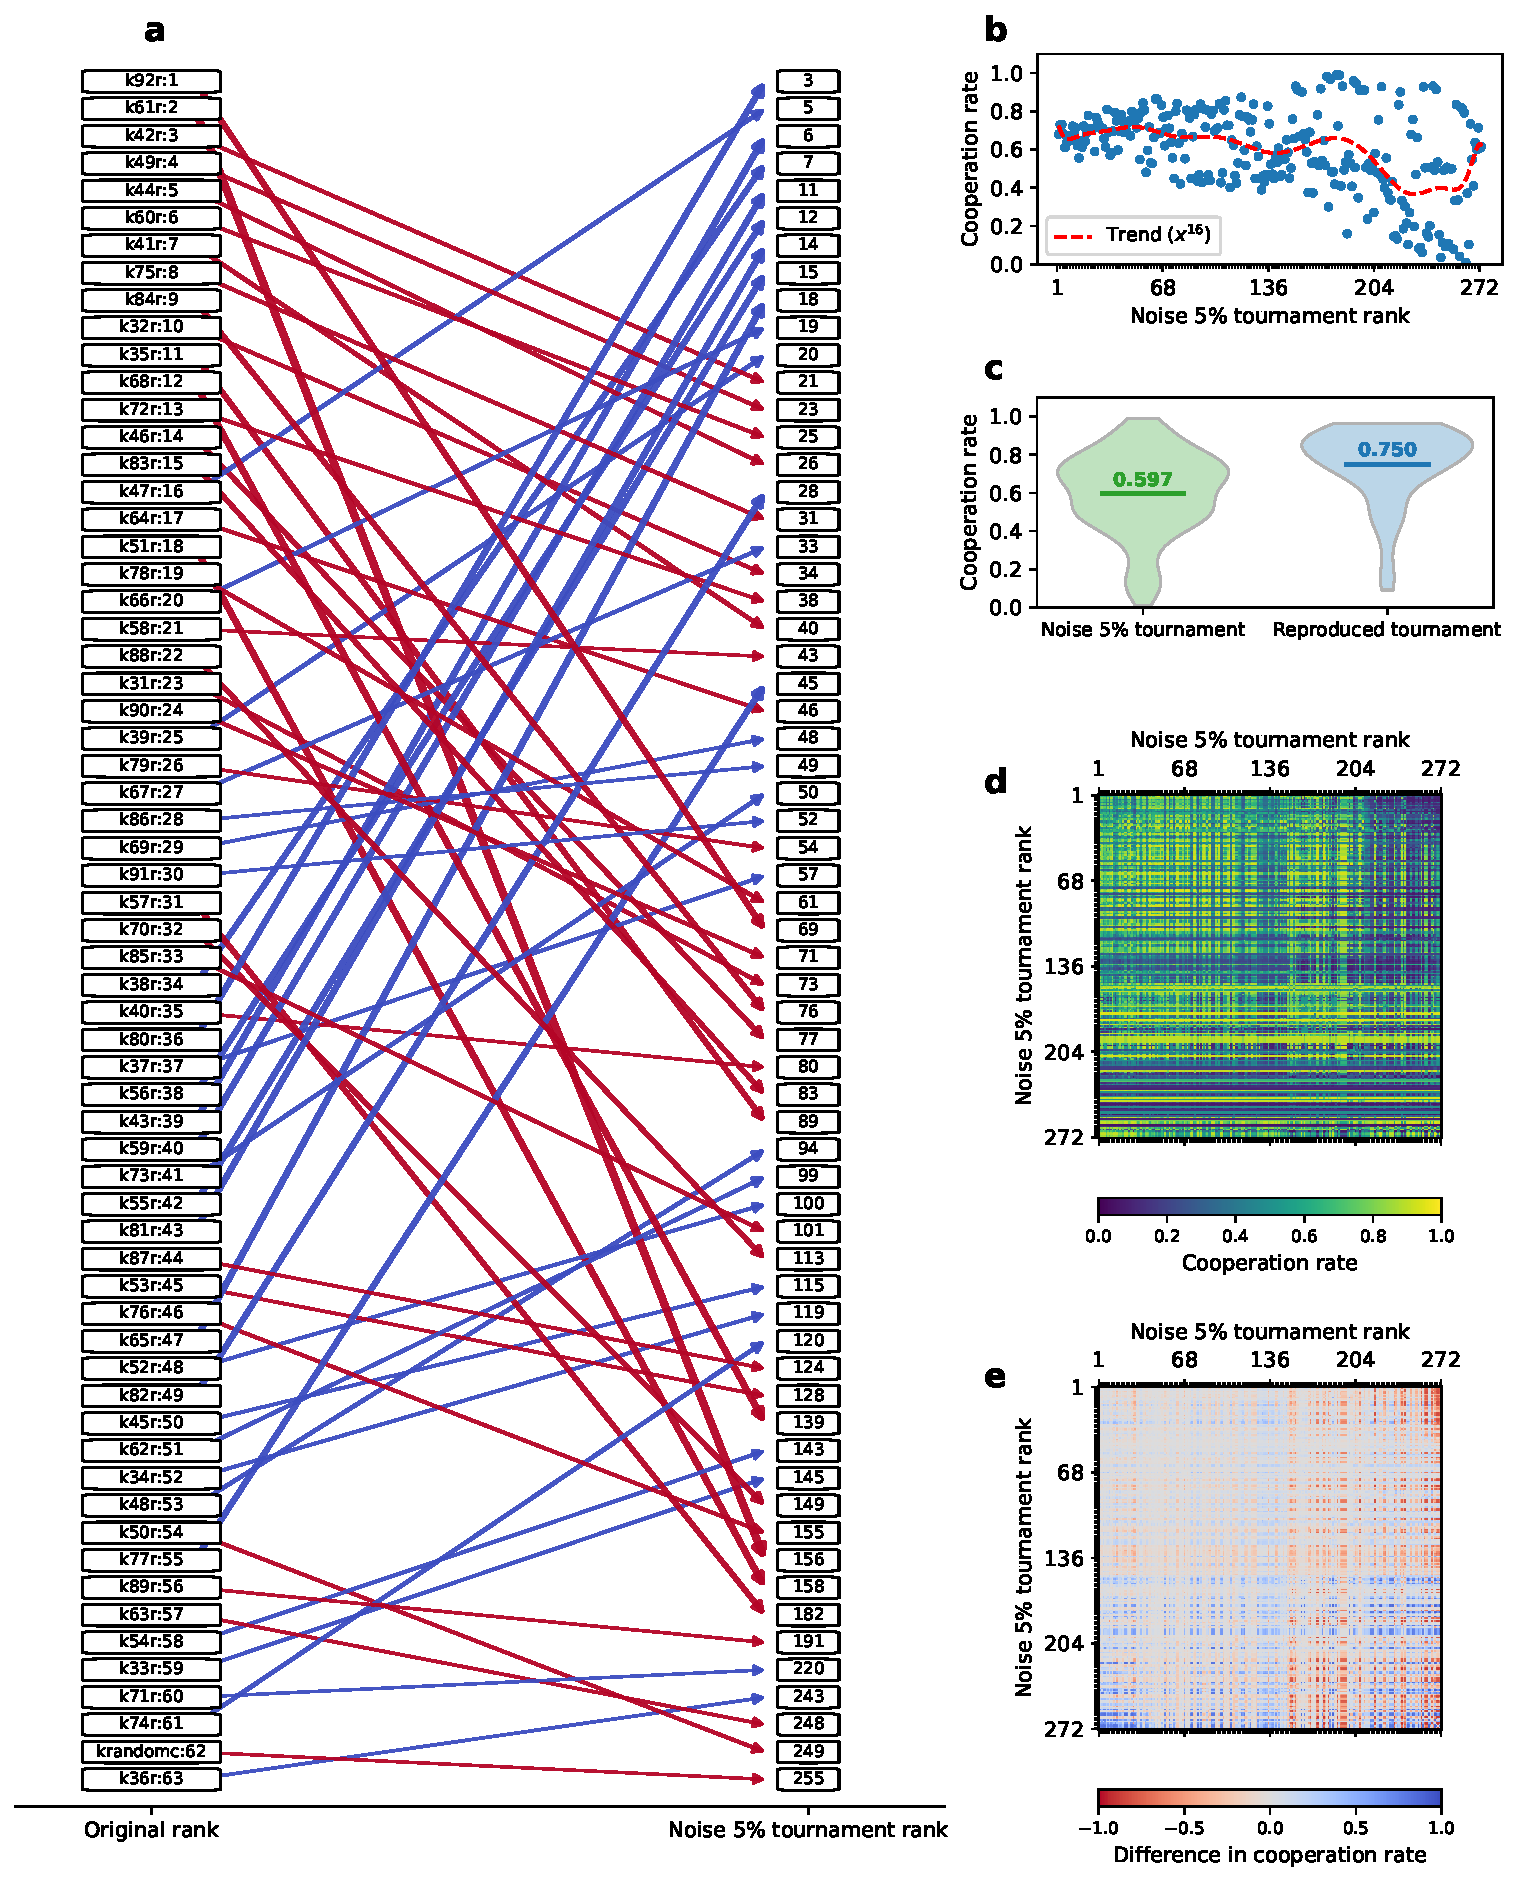
\includegraphics[width=.90\textwidth]{../paper/assets/axelrod_python_tournament_noise_5.pdf}
    \caption{\textbf{Reproduction of Axelrod's second tournament with the addition
    of the strategies from the \AXL{} library and 5\% noise.}
    The panels follow the same layout as
    Supplementary Figure~\ref{fig:axl_noise_1}.
    \textbf{a,} Comparison of the original rankings (left column) and the rankings
    in this tournament (right column), with strategies ordered by their original
    ranks. Arrows indicate the change in rank, with widths proportional to the size
    of the change; blue arrows indicate a positive change in rank, red arrows a
    negative change, and grey arrows no change.
    \textbf{b,} Cooperation rates of strategies ordered by rank in this tournament.
    \textbf{c,} Tournament cooperation rates across all repetitions for this
    tournament (green) and the reproduced tournament without the additional
    strategies (blue); the solid line shows the average cooperation rate.
    \textbf{d,} Pairwise cooperation rates between strategies, ordered by their
    rank in this tournament.
    \textbf{e,} Differences in pairwise cooperation rates, again ordered by rank
    in this tournament.}
    \label{fig:axl_noise_5}
\end{figure}


\section{Fortran source code for k42r}\label{app:k42r_fortran}

From inspection of the 
source code, the behaviour of the strategy can be described as follows 
(these descriptions are taken from the re-implementation in Python 
from~\cite{AxelrodProject}, which has been verified to reproduce the original 
Fortran behaviour accurately):

This player keeps track of the opponent's responses to own behavior:

    \begin{itemize}
        \item \texttt{cd\_count} counts: Opponent cooperates as response to player defecting.
        \item \texttt{cc\_count} counts: Opponent cooperates as response to player cooperating.
    \end{itemize}

The player has a defect mode and a normal mode.  In defect mode, the
player will always defect.  In normal mode, the player obeys the following
ranked rules:

    \begin{enumerate}
        \item If in the last three turns, both the player/opponent defected, then
            cooperate for a single turn.
        \item If in the last three turns, the player/opponent acted differently from
            each other and they're alternating, then change next defect to
            cooperate.  (Doesn't block third rule.)
        \item Otherwise, do tit-for-tat.
    \end{enumerate}

Start in normal mode, but every 25 turns starting with the 27th turn,
re-evaluate the mode.  Enter defect mode if any of the following
conditions hold:

    \begin{itemize}
        \item Detected random:  Opponent cooperated 7-18 times since last mode
evaluation (or start) AND less than 70\% of opponent cooperation was in
response to player's cooperation, i.e.
    \texttt{cc\_count} / (\texttt{cc\_count}+\texttt{cd\_count}) < 0.7
\item Detect defective:  Opponent cooperated fewer than 3 times since last mode
evaluation.
    \end{itemize}

When switching to defect mode, defect immediately. The first two rules for
normal mode require that the last three turns were in normal mode.  When starting
normal mode from defect mode, defect on first move.


\begin{figure}[!hbtp]
    \begin{center}
        \scriptsize
        \begin{lstlisting}[language=Fortran,
                           basicstyle=\ttfamily\tiny,
                           frame=single,
                           keywordstyle=\color{red}\bfseries,
                           commentstyle=\color{teal}\itshape]
       FUNCTION K42R(JPICK,MOVEN,ISCORE,JSCORE,RANDOM, JA)
C BY OTTO BORUFSEN
C TYPED FROM FORTRAN BY AX, 1/25/79
      DIMENSION MHIST(2,2)
      k42r=ja    ! Added 7/27/93 to report own old value
C INITIALIZE FIRST MOVE
      IF(MOVEN.NE.1)GOTO 20
         L3MOV=0
         L3ECH=0
         IDEF=0
         ICOOP=0
         IPICK=0
         DO 10 I=1,2
         DO 10 J=1,2
10       MHIST(I,J)=0
         GO TO 500
20    IF(MOVEN.EQ.2)GOTO 25
C UPDATE MOVE HISTORY
      MHIST(I2PCK+1,JPICK+1)=MHIST(I2PCK+1,JPICK+1)+1
25    IF(IDEF.EQ.0)GOTO 30
C OPPONENT HAS BEEN PROVED "RANDOM" OR
C "DEFECTIVE",I DEFECT FOR 25 MOVES
      K42R=1
      GO TO 100
30    IF(IPICK.EQ.0.OR.JPICK.EQ.0)GOTO 40
C MUTUAL DEFECTIONS ON LAST MOVE.
      L3MOV=L3MOV+1
      IF(L3MOV.LT.3)GOTO 50
C MUTUAL DEFECTION ON
C LAST THREE MOVES.
C I COOPERATE ONCE ON NEXT MOVE.
      K42R=0
      L3MOV=0
      L3ECH=0
      GOTO 100
C ONE (OR BOTH) COOPERATED ON LAST MOVE.
40    L3MOV=0
      IF(IPICK.EQ.JPICK)GOTO 45
      IF(JPICK.NE.I2PCK.OR.IPICK.NE.J2PCK)GOTO 45
C ECHO-EFFECT ON LAST MOVE.
      L3ECH=L3ECH+1
      IF(L3ECH.LT.3)GOTO 50
C ECHO-EFFECT ON LAST THREE MOVES.
C MY NEXT DEFECTION WILL BE SUBSTITUTED
C BY A COOPERATION.
      L3ECH=0
      L3MOV=0
      ICOOP=1
      GOTO 50
45    L3ECH=0
C PLAY 'TIT FOR TAT' AS MAIN RULE.
50    K42R=JPICK
100   IF(MOD(MOVEN-2,25).NE.0.OR.MOVEN.EQ.2)GOTO 650
C ON EVERY 25 MOVES:
C CHECK IF OPPONENT SEEMS TO BE
C 'RANDOM' OR 'DEFECTIVE'.
      IDEF=0
      JNCOP=MHIST(1,1)+MHIST(2,1)
C IS OPPONENT 'RANDOM'?
      IF(JNCOP.GT.17)GOTO 155
      IF(JNCOP.LT.8)GOTO 130
      IF(100*MHIST(1,1)/JNCOP.LT.70)IDEF=1
      GOTO 155
C IS OPPONENT 'DEFECTIVE'?
130   IF(JNCOP.LT.3)IDEF=1
155   DO 160 I=1,2
      DO 160 J=1,2
160   MHIST(I,J)=0
      IF(IDEF.EQ.0)GOTO 650
C OPPONENT SEEMS TO BE
C 'RANDOM' OR 'DEFECTIVE'.
C I DEFECT FOR NEXT 25 MOVES.
      ICOOP=0
      L3MOV=0
      L3ECH=0
      GOTO 600
C I COOPERATE.
500   K42R=0
      GOTO 650
C I DEFECT.
600   K42R=1
650   IF(ICOOP.EQ.0.OR.K42R.EQ.0)GOTO 660
         ICOOP=0
         K42R=0
660   I2PCK=IPICK
      J2PCK=JPICK
      IPICK=K42R
      RETURN
      END
        \end{lstlisting}
        \caption{Fortran Source code for original k42r strategy submitted
        to Axelrod's second tournament.}
        \label{fig:k42r_fortran}
    \end{center}
\end{figure}

\section{List of all strategies}\label{app:list_of_all_players}

Here we list all the strategies including both the original and the ones from
the \AXL{} library. Their ranks are shown as: Rank in full tournament / Rank in
full tournament with 1\% noise / Rank in full tournament with 5\% noise / Rank
in original tournament (if an original strategy).

\begin{multicols}{2}
    \begin{enumerate}
            \input{../paper/assets/list_of_all_players.tex}
    \end{enumerate}
\end{multicols}

\section{Interaction distributions}\label{app:opponents_distributions}

Here we show the distributions of interactions in terms of cooperation rates and
payoffs for both the original tournament and the expanded \AXL{} tournament.

\begin{figure}[!hbtp]
    \begin{center}
        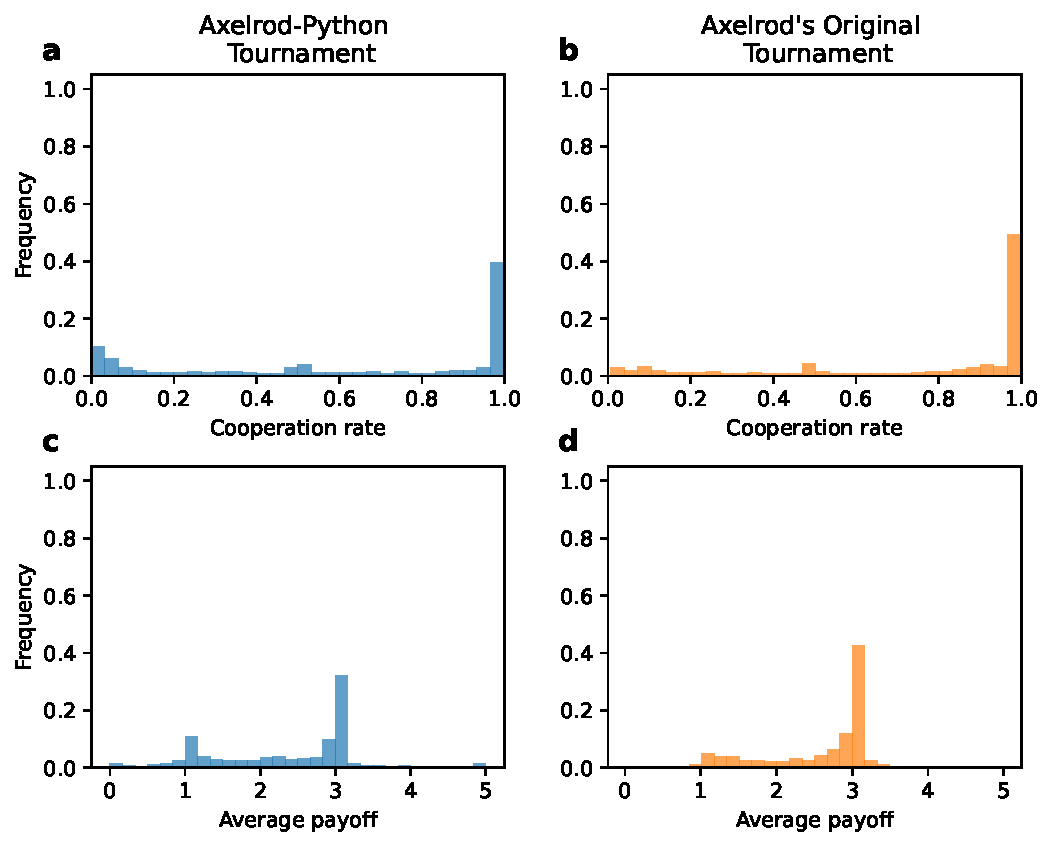
\includegraphics[width=.75\textwidth]{../paper/assets/distribution_of_opponents_comparison.pdf}
        \caption{\textbf{Interaction distributions in the original and \AXL{} tournaments.}
        Distributions of pairwise interaction cooperation rates and payoffs for
        the \AXL{} tournament and the original tournament. The
        cooperation rate distributions are strongly skewed towards one,
        indicating that a large fraction of interactions are highly cooperative.
        In the \AXL{} tournament, however, there is also a visible tail
        close to zero cooperation, indicating the presence of exploitative
        interactions that are largely absent from the original tournament. This
        difference may help explain why highly cooperative strategies such as
        \TFT{} become less effective in more diverse tournaments, where
        strategies capable of exploiting others are more successful. The payoff
        distributions are similarly skewed around mutual cooperation payoffs,
        although noticeable differences between the tournaments remain. Overall,
        these results suggest that the interaction environments induced by the
        tournaments are highly structured rather than uniform across behavioural
        space.}
        \label{fig:original_tournament_interaction_distributions}
    \end{center}
\end{figure}

\section{Probabilistic ending tournament}\label{app:probiblitist_distributions}

Axelrod originally intended the second tournament to use probabilistic match
endings rather than fixed match lengths. However, in practice, for a given
continuation probability, what is described in the paper is that he sampled five different match lengths, and each
pair of strategies used each of these five match lengths once. This is also
the approach we followed when replicating the tournament.

Here, we perform an additional sensitivity analysis to evaluate whether our
results depend sensitively on the precise interpretation of the tournament
stopping rule by considering matches that end probabilistically rather than
after a fixed number of turns.

Specifically, we consider a continuation probability corresponding to an
expected match length of 151 turns. Under this implementation, after each turn
the match continues with probability $150/151$ and ends with probability
$1/151$. We repeat this
full tournament 1000 times. The results are shown in
Supplementary Figure~\ref{fig:probabilistic_ending_tournament}.

Overall, the main conclusions remain unchanged. In particular, TFT ($k92r$)
still ranks first, while $k36r$ remains the lowest-performing strategy.
Although some strategies experience modest rank shifts under probabilistic
endings, these changes are relatively small and remain within the range of
variation already observed when reproducing the tournament using fixed match
lengths.

\begin{figure}[!hbtp]
    \begin{center}
        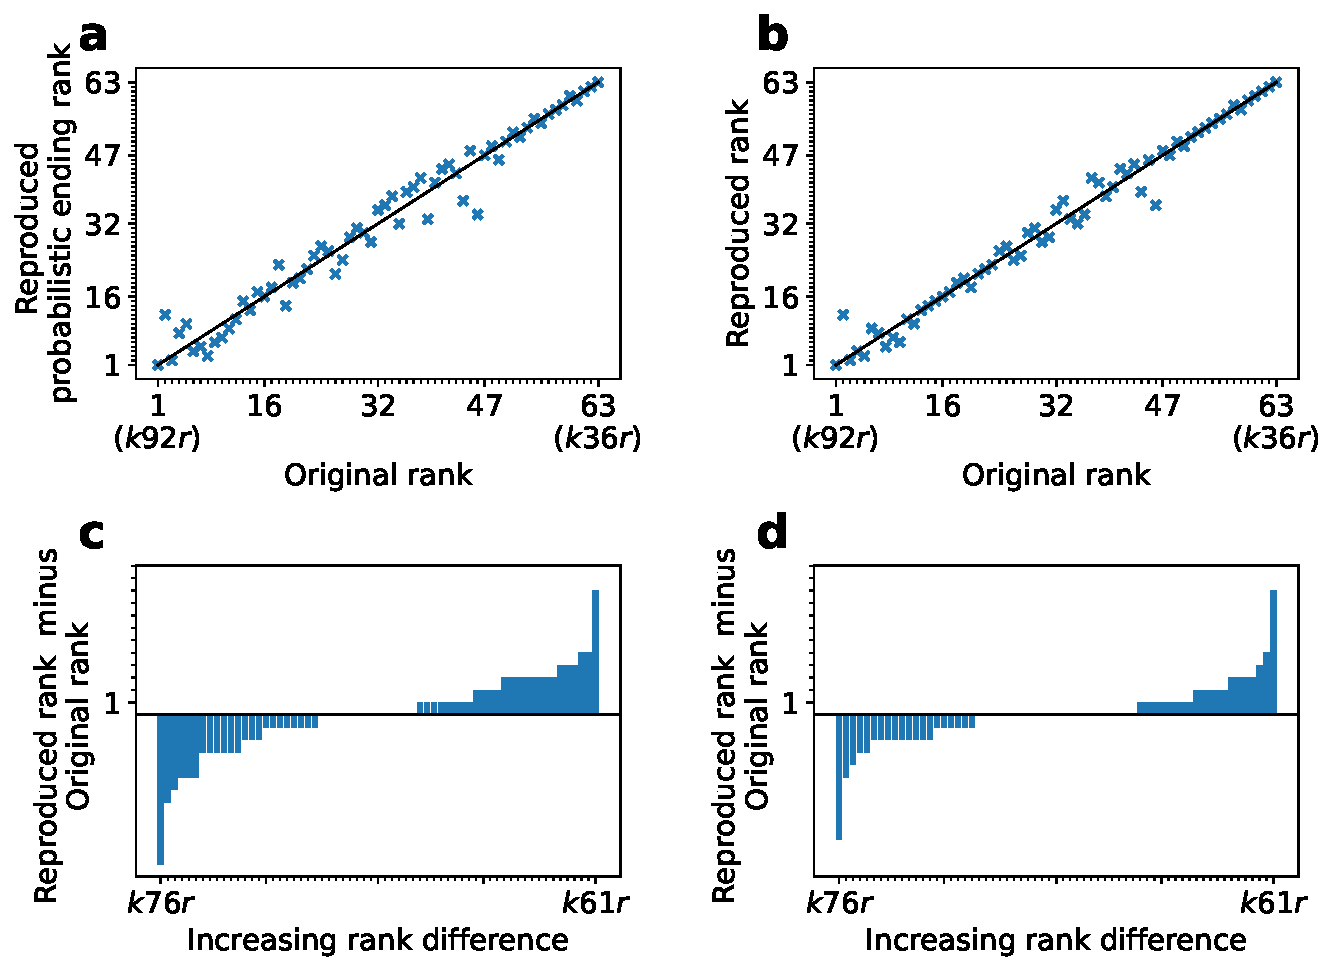
\includegraphics[width=.75\textwidth]{../paper/assets/probalistic_ending_tournament.pdf}
        \caption{
        \textbf{Probabilistic ending tournament.}
        Comparison between the original tournament rankings and reproduced
        rankings under probabilistic and fixed match lengths. Panels~\textbf{a}
        and~\textbf{b} show the reproduced ranks against the original ranks for
        the probabilistic-ending and fixed-length implementations,
        respectively. Panels~\textbf{c} and~\textbf{d} show the corresponding
        rank differences relative to the original tournament. Despite small
        variations for some strategies, the overall tournament structure and
        the identities of the highest- and lowest-ranked strategies remain
        unchanged. Panels~\textbf{b} and~\textbf{d} are also shown in the main
        text (Figure~2); however, we reproduce them here to allow for direct
        comparison with the probabilistic-ending tournament results.
        }
        \label{fig:probabilistic_ending_tournament}
    \end{center}
\end{figure}

\bibliographystyle{naturemag}
\bibliography{../paper/bibliography.bib}

\end{document}
